\documentclass[]{report}

\voffset=-1.5cm
\oddsidemargin=0.0cm
\textwidth = 480pt

\usepackage{framed}
\usepackage{subfiles}
\usepackage{graphics}
\usepackage{newlfont}
\usepackage{eurosym}
\usepackage{amsmath,amsthm,amsfonts}
\usepackage{amsmath}
\usepackage{color}
\usepackage{amssymb}
\usepackage{multicol}
\usepackage[dvipsnames]{xcolor}
\usepackage{graphicx}
\begin{document}
\chapter{Introduction to Normal Distribution}

	\section{Normal Distribution} The normal probability distribution is important in statistical inference for three distinct reasons:
	
	\begin{itemize}
		\item[(1)] The measurements obtained in many random processes are known to follow this distribution.
		\item[(2)] Normal probabilities can often be used to approximate other probability distributions, such as the
		binomial and Poisson distributions.
		\item[(3)] Distributions of such statistics as the sample mean and sample proportion are normally distributed
		when the sample size is large, regardless of the distribution of the parent population.
	\end{itemize}
	As is true for any continuous probability distribution, a probability value for a continuous random variable can be determined only for an interval of values. The height of the density function, or probability curve, for a normally distributed variable is given by an integral formula.
	
	
	
	
	
	\begin{center}
		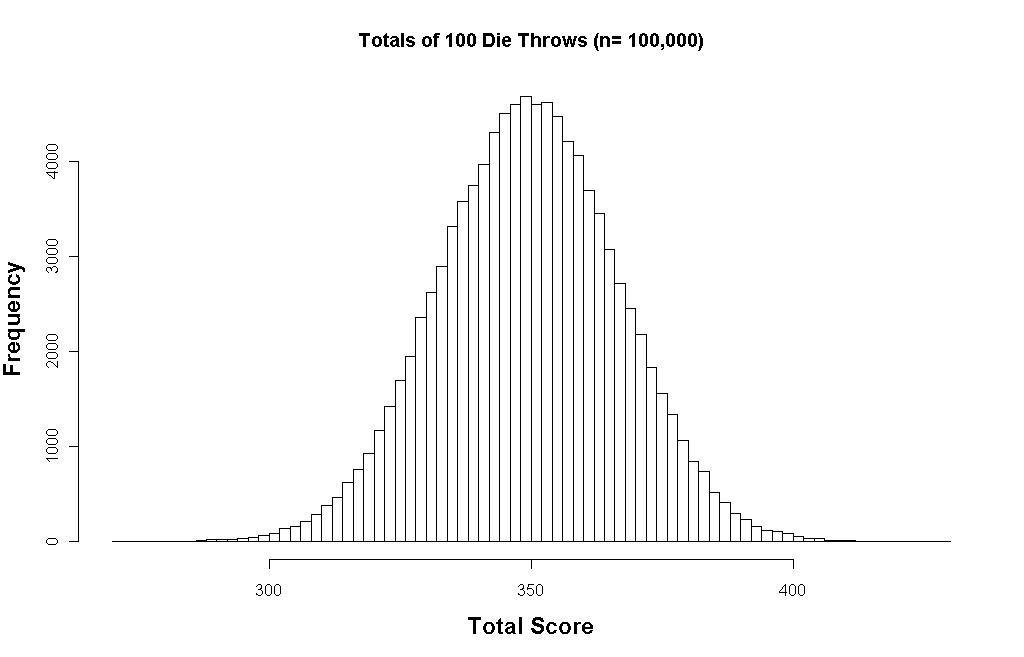
\includegraphics[scale=0.30]{images/3aDieHist3}
	\end{center}

\subsection{Bell Curve}
Bell curves show up throughout statistics. Diverse measurements such as diameters of seeds, lengths of fish fins, scores on the SAT and weights of individual sheets of a ream of paper all form bell curves when they are graphed. The general shape of all of these curves is the same. But all of these curves are different, because it is highly unlikely that any of them share the same mean or standard deviation. Bell curves with large standard deviations are wide, and bell curves with small standard deviations are skinny. Bell curves with larger means are shifted more to the right than those with smaller means.



\begin{itemize}
	\item The normal distribution is perhaps the most widely used distribution for a random variable.
	\item Normal distributions have the same general shape: the bell curve.
	\item They are symmetric with scores more concentrated in the middle than in the tails.
	%\item Examples of normal distributions are shown below. Notice that they differ in how spread out they are. The area under each curve is the same.
	\item The height of a normal distribution can be defined mathematically in terms of two fundamental parameters: the mean ($\mu$) and the standard deviation ($\sigma$).
	\item A normally distributed random variable X is denoted $ X \sim \mbox{N} (\mu, \sigma^2)$ (note that we use the variance term here)
	\item The mean and standard deviation are vital for calculating probabilities.
\end{itemize}

%------------------------------------------------------------------------------------------------%


\section{Dice Roll Experiment Revisited}
	\begin{itemize}
		\item
		Recall the experiment whereby a die was rolled 100 times, and the sum of the 100 values was recorded.
		\item
		This experiment was repeated a very large number of times (e.g. 100,000 times ) in a simulation study.
		\item
		A histogram was drawn to depict the distribution of outcomes of this experiment.
		\item Recall that we agreed that ``bell-shaped" was a good description of the histogram.
		
	\end{itemize}
	
	\section{Exact Probability}
	
	\textbf{Remarks:} This is for continuous distributions only.
	\begin{itemize}
		\item The probability that a continuous random variable will take an exact value is infinitely small.
		We will usually treat it as if it was zero.
		\item
		When we write probabilities for continuous random variables in mathematical notation, we often retain the equality component (i.e. the "...or equal to..").\\
		For example, we would write expressions $P(X \leq 2)$ or $P(X \geq 5)$.
		\item
		Because the probability of an exact value is almost zero, these two expression are equivalent to $P(X < 2)$
		or $P(X > 5)$. \item The complement of $P(X \geq k)$ can be written as $P(X \leq k)$.
	\end{itemize}
	

%=========================================================================%
\subsection{The Complement Rule}
	
	\begin{itemize}
		\item The \textbf{\textit{Complement Rule}} is a very simple rule for working with probability distributions.
		\item In this presentation, we will look at the Complement Rule for continuous probability distributions only.
		
	\end{itemize}
	\begin{itemize}
		
		\item To compute the probability of the complementary event, simple subtract the probability of the event from 1.
		
		\[P(X \leq k) = 1- P(X \geq k) \]
		\[P(X \geq k) = 1- P(X \leq k) \]
	\end{itemize}	
	
	
	
	\begin{framed}
	\noindent \textbf{Important}
	\begin{itemize}
		
	
		\item The probability of being greater than or equal to a value is simply the sum of the probability of being greater than the value and the probability of being equal to the value
		\[  P(X \geq k)  = P( X > k) + P(X = k) \]
			\item Remember, for continuous probability distributions, the probability of an \textbf{exact} value is extremely small, such that it is almost zero.
				\[P(X = k) \approx 0\]
		\item Therefore we neglect the equality components in expressions such as
		$P(X \leq k)$ and $P(X \geq k)$.
		\item In fact we can treat this two expressions as \textbf{\textit{complementary events}}.
	\end{itemize}
	\end{framed}
	
	
	
	
	\[P(X \leq k) = 1- P(X \geq k) \]
	\[P(X \geq k) = 1- P(X \leq k) \]
	\begin{center}
	\begin{tabular}{|c|c|c|c|}
		\hline Event &\phantom{s} Prob.\phantom{s} & Complement Event & \phantom{s} Prob.\phantom{s}\\ 
		\hline $P(X \leq 100)$ & 0.65 &$P(X \geq 100)$  &  \\ 
		\hline $P(Y \geq 80)$ & 0.40 & $P(8 \leq 80)$ &  \\ 
		\hline 
	\end{tabular} 
	\end{center}


	\noindent \textbf{The Complement Rule}


	

	
	
	
	
	
	
	
	\subsection{Mathematical Basis of The Normal Distribution}
	The \textbf{\emph{probability density function}} of the normal distribution is given as
	\[ f(x) = \frac{1}{\sqrt{2\pi\sigma^2}} e^{ -\frac{(x-\mu)^2}{2\sigma^2} } \]
	
	Integrating this formula would allow us to compute probabilities.
	However, we will not use this formula, although we later discuss what a probability density function is.
	

	
	\begin{center}
		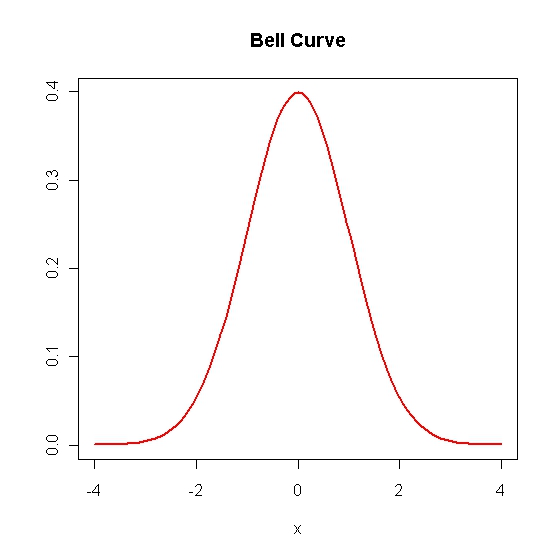
\includegraphics[scale=0.30]{images/5ABellCurve}
	\end{center}
	
\section{Characteristics of the Normal probability distribution}


	\begin{itemize}
		\item[1] The highest point on the normal curve is at the mean, which is also the median and mode of the distribution.
		\item[2] \textbf{[VERY IMPORTANT]}
		The normal probability curve is bell-shaped and symmetric, with the shape of the curve to the left of the mean a mirror image of the shape of the curve to the right of the mean.
		\item[3] The standard deviation determines the width of the curve. Larger values of the the standard deviation result in wider flatter curves, showing more dispersion in data.
		\item[4] The total area under the curve for the normal probability distribution is 1.
	\end{itemize}
	

%------------------------------------------------------------------%
{
	\subsection{ Characteristics of the Normal probability distribution}
	\begin{itemize}
		\item The interval defined by the mean $ \pm 1 \times $ standard deviation includes approximately $68\%$ of the observations, leaving $16\%$ (approx) in each tail.
		\item The interval defined by the mean $ \pm 1.96 \times $ standard deviation includes approximately $95\%$ of the observations, leaving $2.5\%$ (approx) in each tail.
		\item The interval defined by the mean $ \pm 2.58 \times $ standard deviation includes approximately $99\%$ of the observations, leaving $0.5\%$ (approx) in each tail.
	\end{itemize}
	\textbf{Remark:} It is useful to know this numbers, but we will do all calculations from first principles.
}
	

	\subsection{Characteristics of the Normal probability distribution}
	\textbf{Remark:} It is useful to know the following statements as rules of thumb, but we will do all relevant calculations from first principles. However, in an exam situation, these rules of thumb may be invoked, and it is required to show your workings.
	\begin{itemize}
		\item The interval defined by the mean $ \pm 1 \times $ standard deviation includes approximately $68\%$ of the observations, leaving $16\%$ (approx) in each tail.
		\item The interval defined by the mean $ \pm 1.645 \times $ standard deviation includes approximately $90\%$ of the observations, leaving $5\%$ (approx) in each tail.
		\item The interval defined by the mean $ \pm 1.96 \times $ standard deviation includes approximately $95\%$ of the observations, leaving $2.5\%$ (approx) in each tail.
		
		\item The interval defined by the mean $ \pm 2.58 \times $ standard deviation includes approximately $99\%$ of the observations, leaving $0.5\%$ (approx) in each tail.
	\end{itemize}
	
	
	
	Collectively, these points are known as the empirical rule or colloqiuly the \textbf{68-95-99 rule}. Clearly, given a normal distribution, most outcomes will be within 3 standard deviations of the mean.
	
	

	
\section{The Standard Normal Distribution}

Since every different combination of m and s would generate a different normal
probability distribution, tables of normal probabilities are based on one
particular distribution: the standard normal distribution. This is the normal probability distribution with $\mu=0$
and $\sigma=1$. Any value X from a normally distributed population can be converted into the equivalent standard
normal value Z (i.e. a `Z value') by the formula
\[ Z = \frac{X - \mu}{\sigma}\]


\begin{itemize}
	\item The standard normal distribution has been tabulated (usually in the form of value of the cumulative distribution function F), and the other normal distributions are the simple transformations, as described above, of the standard one. \item Therefore, one can use tabulated values of the cdf of the standard normal distribution to 
	find values of the cdf of a general normal distribution.
\end{itemize}



	

%% Section 4.3.1  
%% The normal probability distribution
The form, or shape, of the normal distribution is the bell shaped curve we met in section 2.
The probability density function that defines the bell-shaped curve if the normal distribution is given by




\[f(x \; | \; \mu, \sigma) = \frac{1}{\sigma\sqrt{2\pi} } \; e^{ -\frac{(x-\mu)^2}{2\sigma^2} }\]

where 

\begin{itemize}
	\item $\mu$ = expected value, or mean, of the random variable x.
	\item $\sigma$  = standard deviation of the random variable x.
\end{itemize}
[Remark - We will never be using this formula]
%=========================================================5












\section{Rules of Thumb}
Additionally, every normal curve (regardless of its mean or standard deviation) conforms to the following "rule".

\begin{itemize}
	\item About $68\%$ of the area under the curve falls within 1 standard deviation of the mean.
	\item About $95\%$ of the area under the curve falls within 2 standard deviations of the mean.
	\item About $99.7\%$ of the area under the curve falls within 3 standard deviations of the mean.
\end{itemize}
\textbf{5) Useful Rules of Thumb.}

\begin{itemize}
	\item	The mean $\pm$  1 standard deviation includes 68\% of the observations ,leaving 16\% (approx) in each tail.
	
	\item	The mean $\pm$  1.96 standard deviation includes 95\% of the observations ,leaving 2.5 \% (approx) in each tail.
	
	\item 	The mean $\pm$  2.58 standard deviation includes 99\% of the observations ,leaving 0.5 \% (approx) in each tail.
\end{itemize}


Collectively, these points are known as the empirical rule or colloqiuly the \textbf{68-95-99 rule}. Clearly, given a normal distribution, most outcomes will be within 3 standard deviations of the mean.





%---------------------------------------------------%

%\frametitle{Normal Distribution : The Symmetry Rule}


Consider the normally distributed random variable $X$

\[ X \sim \mathcal{N}(\mu=1000,\sigma^2 = 2500) \]

Paramters:
\begin{itemize}
	\item $\mu =1000$
	\item $\sigma =50$
\end{itemize}
Questions

\begin{itemize}
	\item $P(X \leq 925)$
	\item $P(X \geq 925)$
\end{itemize}



%---------------------------------------------------%

%\frametitle{Normal Distribution : The Symmetry Rule}
\textbf{Z-score}
\[ z =\frac{x - \mu}{\sigma}\]
%------------------------------------------------------------------------------------------------%


\section{Three Important Rules for the Normal Distribution}


\subsection{Normal Distribution : The Symmetry Rule}

From statistical tables, we could determine the following:
\begin{itemize}
	\item $P(Z \leq 1.5) $
	\item $P(Z \geq 1.5) $
\end{itemize}



As a consequence of Property 1, it is possible to relate all normal random variables to the standard normal.

If $X \sim N(\mu, \sigma^2)$, then

\[Z = \frac{X - \mu}{\sigma} \]
is a standard normal random variable: $Z \sim N(0,1)$. An important consequence is that the cdf of a general normal distribution is therefore

\[\Pr(X \le x)
=
\Phi
\left(
\frac{x-\mu}{\sigma}
\right)
=
\frac{1}{2}
\left(
1 + \operatorname{erf}
\left(
\frac{x-\mu}{\sigma\sqrt{2}}
\right)
\right)\]
.





%-------------------------------------------------------------------------%



Conversely, if Z is a standard normal distribution, $Z \sim N(0,1)$, then

\[X = \sigma Z + \mu\]
is a normal random variable with mean $\mu$ and variance $\sigma^2$.






\subsection{The Normal Distribution: Symmetric Intervals}


Symmetric Intervals

\[ P( -z \leq Z \leq z) \]

	








\newpage

%------------------------------------------------------------------------%
{
	\textbf{Using the Murdoch Barnes Tables}
	
	
	\begin{itemize}
		\item Knowing the Z value is very useful, because it is easy to compute $P(Z \geq Z_0)$ for some value $Z_0$ using statistical tables.
		\bigskip
		\item $P(X \geq X_0) = P(Z \geq Z_0)$\bigskip
		\item From our previous example we can say the following
		\[ P(X \geq 100) = P(Z \geq 2.5)\]
	\end{itemize}
	
}


{
	\textbf{Normal Distribution} 
	\begin{itemize}
		\item Normal distributions are a family of distributions that have the same general shape. 
		\item They are symmetric with scores more concentrated in the middle than in the tails. Normal distributions are sometimes described as bell shaped. 
		\item Examples of normal distributions are shown below. Notice that they differ in how spread out they are. The area under each curve is the same. 
		\item The height of a normal distribution can be specified mathematically in terms of two parameters: the mean ($\mu$) and the standard deviation ($\sigma$). 
		
	\end{itemize}
}






	

		
		

	
	

	
	%{
	%\subsection{Using Murdoch Barnes Tables 3}
	%
	%Find $ P(Z \geq 1.64)$ and $ P(Z \geq 1.65)$.\\\bigskip Which row and column?
	%\begin{itemize}
	%\item 1.64 = \color{blue}{1.6}+\color{orange}{0.04} \color{black}\hspace{2cm}$ P(Z \geq 1.64) =0.0505$
	%\item 1.65 = \color{blue}{1.6}+\color{green}{0.05}  \color{black} \hspace{2cm}$ P(Z \geq 1.65) =0.0495$
	%\end{itemize}
	%\bigskip
	%\small
	%\begin{table}[ht]
	%%\caption{Standard Normal Distribution } % title of Table
	%\centering % used for centering table
	%\begin{tabular}{|c|| c c c c c c|} % centered columns (4 columns)
	%\hline %inserts double horizontal lines
	%& & \ldots & \color{orange}{0.04} & \color{green}{0.05} &0.06&0.07\ldots \\
	%%heading
	%\hline \hline% inserts single horizontal line
	%\ldots & \ldots &\ldots &\ldots& \ldots &\ldots&\ldots \\ %Checked
	%1.5 & \ldots & 0.0630&0.0618& 0.0606 &0.0594&\dots \\ % inserting body of the table
	%\color{blue}{1.6} & \ldots &0.0516& \alert{0.0505} & \alert{0.0495} &0.0485&\ldots\\
	%1.7 & \ldots &0.0418 &0.0409& 0.0401 &0.0392&\dots \\ % inserting body of the table
	%\ldots & \ldots &\ldots &\ldots& \ldots &\ldots&\ldots \\ %Checked
	%\hline %inserts single line
	%\end{tabular}
	%%\label{table:nonlin} % is used to refer this table in the text
	%\end{table}
	%}
	
	%--------------------------------------------------------%
	
	
	\subsection{Probability Density Function}
	Recall: As the Normal distribution is a continuous distribution, the PDF for a particular observed value will not give us an intuitive
	result (as far as this module is concerned). It is, in fact, the height of the density curve at a particular point.
	
	Nonetheless, the relevant \texttt{R} code may be included in exam questions, so as to add complexity to questions.
	
	\begin{verbatim}
	> dnorm(0.7)
	[1] 0.3122539
	>
	> dnorm(1.7)
	[1] 0.09404908
	
	\end{verbatim}
	
	%------------------------------------------%
	
	\section{Sample Question}
	Suppose $X$ is a normally distributed random variable with mean $\mu = 2000$ and standard deviation $\sigma=200$.
	Compute the probability of X being less than (or equal to) 2340.
	
	\[P(X \leq 2340)\]
	
	As always, we compute the z-score that corresponds to 2340.
	\[ z_o = \frac{x_o - \mu}{\sigma}  = \frac{2340-2000}{200} = 1.7\]
	
	%------------------------------------------%
	
	
	\subsection{\texttt{R} Implementation}
	
	
	Using the following \texttt{R} code, we can determine $P(Z \leq 1.7)$.
	\begin{verbatim}
	
	> pnorm(1.7)
	[1] 0.9554345
	
	\end{verbatim}
	
	
	%------------------------------------------%
	
	
	\subsection{Direct \texttt{R} Implementation}
	
	This can easily be implemented directly - without using the standardization formula, by specifying the normal mean and normal standard deviation directly. However, we will not be using this approach in this module.
	\begin{verbatim}
	
	> pnorm(2340,mean=2000,sd=200)
	[1] 0.9554345
	
	
	\end{verbatim}
	
	
	
	
	
	
	
	
	
	\section{Solving using the Z distribution}
	When we have a normal distribution with any mean   and any standard deviation  , we answer probability questions about the distribution by first converting all values to corresponding values of the standard normal ("z") distribution. 
	
	The formula used to convert any random variable "X" ( with mean $\mu$  and standard deviation $\sigma$  specified)  to the standard normal ("Z") distribution is given as follows. 
	\[Formula\]
	
	is the standard normal random variable with a mean of zero and a standard deviation of 1. 
	
	It can be thought of as a measure of how many standard deviations that a value "x" is from mean  .
	
	%=======================================================================%
	
	
	Remarks
	
	A value of x equal to mean   results in a z -value of 0
	
	
	Thus we can see that a value of "x" corresponding to its mean    corresponds to a z-value at its mean , which is 0.
	
	A value of "x" that is one standard deviation above its mean (i.e.  ), we see that the corresponding z value is 1.
	
	
	Thus a value of x that is one standard deviation away from it's mean yields a z-value of 1.
	
	%=======================================================================%
	
	
	Example
	Given that the mean   = 100 and that the standard deviation    = 2.5, what is the "z-value" for normal random variable x = 106?
	
	
	
	Relationship between "x value" and "z  value"
	
	[VERY IMPORTANT]
	
	If    (   and   are some values )
	
	then  
	
	
	By extension  
	
	
	From previous example 
	
	
	
	From Murdoch Barnes Table 3, 
	
	
	
	
	Therefore 
	
	%=======================================================================%
	
	[Finish] 
	
	
	
	
	
	
	
	
	\section{The Complement Rule}
	
	\begin{itemize}
		\item The \textbf{\textit{Complement Rule}} is a very simple rule for working with probability distributions.
		\item In this presentation, we will look at the Complement Rule for continuous probability distributions only.
		
	\end{itemize}
	\begin{itemize}
		
		\item To compute the probability of the complementary event, simple subtract the probability of the event from 1.
		
		\[P(X \leq k) = 1- P(X \geq k) \]
		\[P(X \geq k) = 1- P(X \leq k) \]
	\end{itemize}	
	
	
	
	\begin{framed}
		\subsection{Important}
		\begin{itemize}
			
			
			\item The probability of being greater than or equal to a value is simply the sum of the probability of being greater than the value and the probability of being equal to the value
			\[  P(X \geq k)  = P( X > k) + P(X = k) \]
			\item Remember, for continuous probability distributions, the probability of an \textbf{exact} value is extremely small, such that it is almost zero.
			\[P(X = k) \approx 0\]
			\item Therefore we neglect the equality components in expressions such as
			$P(X \leq k)$ and $P(X \geq k)$.
			\item In fact we can treat this two expressions as \textbf{\textit{complementary events}}.
		\end{itemize}
	\end{framed}
	
	
	
	

	
	
	
	
	
	
	
	
	
	
	
	
	
	
	
	
	



\subsection*{Parameter Values}

Given the parameters of the normal distribution $X$ in the question.
\begin{itemize}
	\item Normal Mean $\mu = 73$ points
	\item Normal Standard Deviation $\sigma = 8$ points
\end{itemize}

\begin{itemize}
	\item $P(X \leq 91)$
	\item $P(65 \leq X \leq 89)$
\end{itemize}

\noindent \textbf{Solutions}
\begin{itemize}
	\item Find the Z score for X = 91.
	
	\[ Z = \frac{x- \mu}{ \sigma} = \frac{91 - 73}{8} =\frac{18}{8} = 2.25\]
	\item Therefore we can say :\\ $P(X \leq 91)$ = $P(Z \leq 2.25)$ \\
	
	
\item From the tables $P(Z \leq 2.25) = 0.9877$
Therefore the probability of getting a grade lower than 91 is 0.9877 (i.e 98.77\%)


\item What is the probability of getting a score between 65 and 89.
Writing this mathematically:
\[ P(65 \leq X \leq 89) \]
\end{itemize}




%================================================================%
\begin{itemize}
\item How many people get a score greater than 89? ($P(X\geq 89)$)
\item How many people get a score less than 65? ($P(X\leq 65)$)
\end{itemize}

To compute $P(X \geq 89)$ first compute the Z-score.

\[ Z = \frac{x - \mu}{\sigma} = \frac{89 - 73}{8} =\frac{16}{8} = 2 \]

$P(X \geq 89)$ = $P(Z \geq 2)$ = 0.0225.

To compute $P(X \leq 65)$ first compute the Z-score.

\[ Z = \frac{x - \mu}{\sigma} = \frac{65 - 73}{8} =\frac{-8}{8} = -1 \]

$P(X \leq 65)$ = $P(Z \leq -1)$ 

\begin{itemize}
\item We use the \textbf{symmetry rule}
\[ P(Z \leq -1) = P(Z \geq +1) \]
\item so we can say $P(X \leq 65)$ = $P(Z \geq +1)$ 
\item From the statistical tables $P(Z \geq +1)$ = 0.1583.
\end{itemize}







\section{Normal Distribution: Worked Examples}

% % MA4413    Computer Maths 3     January 2007
% % Q5. a) 
Assume that the amount of wine poured into a bottle has a normal distribution with a mean of 750ml and a variance of 144ml$^2$.

\begin{itemize}

\item[(i)]  Calculate the probability that a bottle contains more than 765ml. (2 marks)
\item[(ii)]    Calculate the probability that a bottle contains between 744ml and 759ml. (3 marks)
\end{itemize}
%=========================================================== %
A machine fills bags with animal feed. The nominal weight of a bag is 50kg.
Because random variations the weight of a filled bag is normally distributed
$N(\mu, \sigma^2)$. The variance ($\sigma^2$) is known to be 0.01kg$^2$ and $\mu$ is set by the
operator to a particular value.

\begin{itemize}
\item[(i)] If ? = 50kg calculate the probability of a bag containing less than
49.95kg?
\item[(ii)] Calculate the value of "?" such that only $2\%$ of the output are under the
nominal weight?
\end{itemize}




%--------------------------------------------------------------------------- %

\subsection{The Normal Distribution}

{
\normalsize
Key Parameters of the Normal Distribution
\begin{itemize}
\item Normal Mean $\mu$ \\(pronounced ``mu")
\item Normal Standard Deviation $\sigma$ \\ (pronounced ``sigma")
\end{itemize}

\begin{itemize}
\item Suppose we are interested in a normally distributed variable called $X$ (for example: Heights or Weights).
\item We are given specific values for 
\\  - Normal Mean $\mu$ 
\\  - Normal Standard Deviation $\sigma$ 
\end{itemize}
}





\subsection{The Normal Distribution}



$X$ = Weights
\bigskip
\begin{itemize}
\item Mean of X:  $\mu$ = 1000 kg 
\item Standard Deviation of X : $\sigma$ = 20 kg
\end{itemize}
\bigskip

Compute the z-score for 1050 kgs and 985 kgs



\subsection{The Normal Distribution :  Exercise 1}

\[ z_o = \frac{x_o - \mu}{\sigma}  \]
($x_o$ = 1050 kgs, $\mu = 1000$ kgs, $\sigma$ = 20 kgs)



\subsection{The Normal Distribution :  Exercise 2}

\[ z_o = \frac{x_o - \mu}{\sigma}  \]
($x_o$ = 985 kgs, $\mu = 1000$ kgs, $\sigma$ = 20 kgs)









\newpage
\section{Exam Score Example}
The distribution of the exam scores in a statistics distribution is normally distributed with mean $\mu=45$  and standard deviation 
$\sigma=16$
.

You receive a mark of 49.
\begin{itemize}
\item[(i)]
What is the probability of someone scoring higher than you?

\item[(ii)] What percentage of people scored above the mean but lower than you?
\end{itemize}
%-------------------------------------------------------%
Solution to part 1

Let $X$ be the score variable in the statistics exam

$P(X \geq 49)$ 

1) Find the  "z-value" corresponding to a score of 49 , given that mean $mu=45$   and standard deviation  $\sigma=16$ .

\[ z  = \frac{x-\mu}{\sigma}   = \frac{49-45}{16}  = \frac{4}{16} =0.25\]

By definition  

2) From Murdoch Barnes table 3 we can find out the value of   . 

note  0.25 = 0.2 + 0.05

\begin{itemize}
\item    The row is 0.2
\item    The column is 0.05
\end{itemize}
\[
\begin{array}{|c|c|c|c|c|c|c|}\hline
& ....& 0.04& 0.05 & 0.06& .... \\ \hline
0.0&&& 0.4801 & & \\ \hline
0.1&&& 0.4404 && \\ \hline
0.2&&& 0.4013 && \\ \hline
....&&& & &\\ \hline

\end{array} \]

so  

%===================================================================%

Solution to part 2

If  the probability of scoring higher than you is 0.4013, the probability of scoring lower than you is 0.5987  
(from the complement rule , 1 - 0.4013 )


%--------------------------------------------------------------
\newpage
\section{Normal Distribution : Worked Examples}

Remark : This document will be emailed to the class later today.


Important points from yesterday's class.

\begin{itemize}

\item[(i)] Using Murdoch Barnes Table 3 to find   for some value k

\item[(i)] The Complement and Symmetry Rule

Complement   

(only for continuous random variables)

Symmetry   

\item[(i)] Computing "z -values" using the conversion formula.



where   and   are values
\item[(i)] Relationship between "x value" and "z  value"
If    

then  

\end{itemize}
%===================================================================%





\end{document} 
